\section{Auswertung}
\label{sec:Auswertung}

\subsection{Untersuchung der Filterkurve}

Zunächst wird die Durchlassfrequenz $\nu$ des Selektivverstärkers bestimmt. Die 
gemessenen Wertepaare von Frequenz $\nu$ und Spannung $U_\text{A}$ sind in 
Tabelle \ref{tab:Messdaten1} aufgeführt. 

\begin{table}
\centering
\caption{Messwerte der Filterkurve des Selektivverstärkers.}
\label{tab:Messdaten1}
\sisetup{table-format=2.1}
\begin{tabular}{c c c c}
\toprule
$\nu \,/\, \si{\kilo\hertz}$ & $U_\text{A} \,/\, \si{\milli\volt}$ & $\nu \,/\, \si{\kilo\hertz}$ & $U_\text{A} \,/\, \si{\milli\volt}$\\
\midrule
20,0 &  0,865 & 34,6 & 35,00\\
21,0 &  0,900 & 34,7 & 43,00\\
22,0 &  0,990 & 34,8 & 55,00\\
23,0 &  1,095 & 34,9 & 72,50\\
24,0 &  1,230 & 35,0 & 93,00\\
25,0 &  1,380 & 35,1 & 96,00\\
26,0 &  1,560 & 35,2 & 78,00\\
27,0 &  1,800 & 35,3 & 59,00\\
28,0 &  2,100 & 35,4 & 46,00\\
29,0 &  2,520 & 35,5 & 37,00\\
30,0 &  3,200 & 35,6 & 31,00\\
31,0 &  4,000 & 35,7 & 26,00\\
32,0 &  5,450 & 35,8 & 23,00\\
33,0 &  8,350 & 35,9 & 20,00\\
34,0 & 16,000 & 36,0 & 18,00\\
34,1 & 17,000 & 36,1 & 16,00\\
34,2 & 19,500 & 37,0 &  9,00\\
34,3 & 22,000 & 38,0 &  6,15\\
34,4 & 25,000 & 39,0 &  4,60\\
34,5 & 29,000 & 10,0 &  3,70\\
\bottomrule
\end{tabular}
\end{table}

Die gemessene Frequenz $\nu$ wird gegen die Spannung $U_\text{A}$ aufgetragen. Das 
Ergebnis ist in Abbildung \ref{fig:plot1} zu finden. 

\begin{figure}
  \centering
  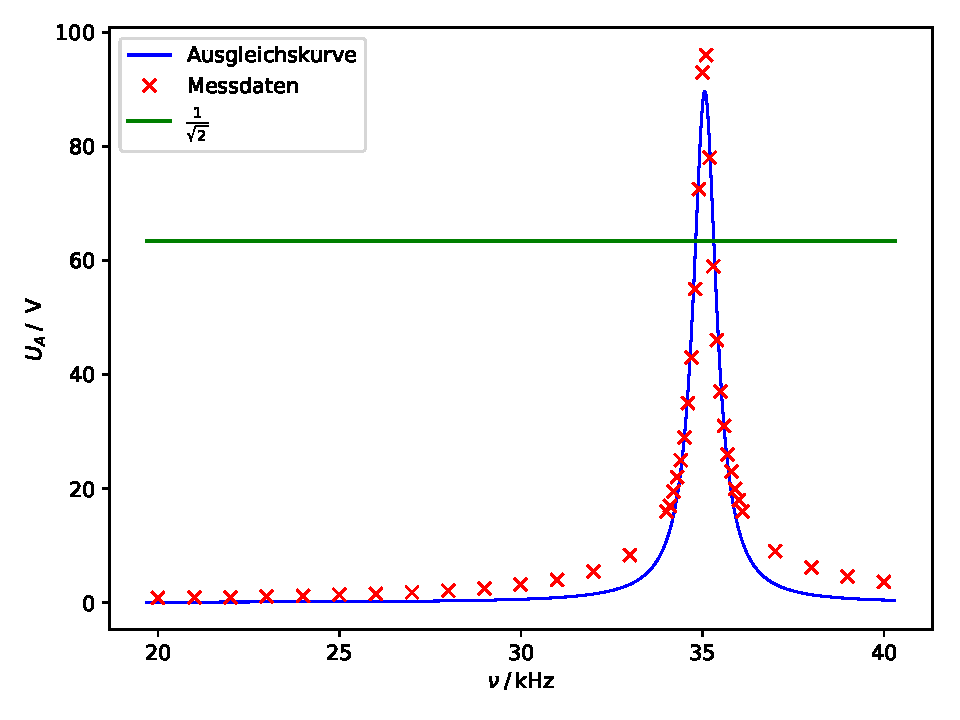
\includegraphics{content/plot1.pdf}
  \caption{Filterkurve des Selektivverstärkers.}
  \label{fig:plot1}
\end{figure}

Mittels Python 3.6.5. und dem Paket Matplotlib wird eine Lorentzkurve für eine Ausgleichskurve 
gefittet. Dabei wird die Gleichung 

\begin{equation*}
f(x) = \frac{a}{(x²-x_0^2)²+\gamma²x_0²}
\end{equation*}

für die berechnete Lorentzkurve und die Werte von $\SI{34.1}{\kilo\hertz}$ bis $\SI{36.0}{\kilo\hertz}$verwendet. 

Die Durchlassfrequenz lässt sich nun direkt ablesen und ergibt sich zu:

\begin{equation}
x_0 = \nu _\text{A} = \SI{35.065}{\kilo\hertz}.
\end{equation}

Desweiteren wird bei einem Wert von $\frac{1}{\sqrt{2}}$ des Maximalwerts
eine Gerade angelegt. Die Parameter ergeben sich schließlich zu: 

\begin{align*}
a &= \SI{6.6+-0.4e4}{\volt\per\second⁴},\\
\gamma &= \SI{0.772+-0.03}{1\per\second²}.
\end{align*}

Außerdem werden $\nu_\text{A}$, $\nu_1$ und $\nu_2$ mittels Python zu

\begin{align*}
\nu_1 &= \SI{34.816+-0.01}{\kilo\hertz},\\
\nu_\text{A} &= \SI{35.065+-0.01}{\kilo\hertz},\\
\nu_2 &= \SI{35.313+-0.01}{\kilo\hertz}
\end{align*}

berechnet. Die Güte $Q$ kann nun mit 

\begin{equation*}
Q = \frac{\nu_\text{A}}{\nu_2 - \nu_1}
\end{equation*}

zu 

\begin{equation*}
Q = \num{70.5+-2.8}
\end{equation*}

berechnet werden.
Der Fehler ergibt sich dabei durch eine Fehlerrechnung mittels 
Python.

\subsection{Theoretische Bestimmung der Suszeptibilitäten}

Nach Formel \eqref{eqn:theo} lassen sich die Theoriewerte Seltener 
Erde Verbindungen berechnen. Es werden $\symup{Dy_2O_3}$, $\symup{C_6O_{12}Pr_2}$, 
$\symup{Gd_2O_3}$ und $\symup{Nd_2O_3}$ untersucht. Es wird eine Temperatur von 
$T = \SI{294}{\kelvin}$ angenommen, was etwa Raumtemperatur entspricht.
Der Lande-Faktor $g_J$, sowie $S$, $L$ und $J$ sind in Tabelle \ref{tab:theo} 
aufgeführt.\\
Die Berechnung der Werte $S$, $L$ und $J$ erfolgt mittels der Betrachtung 
der Anzahl der 4f-Elektronen. Je nach deren Anzahl, gibt es verschieden 
viele Möglichkeiten die Spins in den Elektronen anzuordnen. Diese sollen
unter dem Pauli-Prinzip maximiert werden. Dieses besagt, dass zwei Elektronen
in einem Atom nicht in allen Quantenzahlen übereinstimmen können. \\
Es wird das Molekül $\symup{Dy_2O_3}$ beispielhaft betrachtet. Dieses hat 
$\num{9}$-4f-Elektronen. Auf grundlage des Pauli-Prinzips ergibt sich die 
Hund'sche Regel, welche liefert: $L = -3-2-1+0+1 = -5$. Da der Betrag betrachtet 
wird, nehmen wir $L = 5$ an. $S$ ergibt sich dann mit 
$S = \frac{1}{2}\cdot 7 - \frac{1}{2}\cdot 2 = \num{2.5}$. Zuletzt wird schließlich
$J= L - S = \frac{9}{2} = \num{4.5}$ berechnet. 

\begin{table}
\centering
\caption{Theoretische Werte zur Berechnung der Suszeptibilitäten}
\label{tab:theo}
\sisetup{table-format=2.1}
\begin{tabular}{c c c c c}
\toprule
& $\symup{Nd_2O_3}$ & $\symup{Gd_2O_3}$ & $\symup{Dy_2O_3}$ & $\symup{C_6O_{12}Pr_2}$\\
\midrule
4f-Elektronen                             & 3      & 7      & 9      & 3\\
L                                         & 6      & 0      & 5      & 5\\
S                                         & 1,5    & 3,5    & 2,5    & 1\\
J                                         & 4,5    & 3,5    & 7,5    & 4\\
$g_J$                                     & 0,73   & 2,0    & 1,33   & 0,73\\
$\rho \, / \, \si{\kilo\gram\per\meter³}$ & 7240   & 7400   & 7800   & 6260\\
$m \, / \, \si{\kilo\gram}$               & 0,0090 & 0,0141 & 0,0151 & 0,0079\\
\bottomrule
\end{tabular}
\end{table}


Außerdem ergibt sich $N$ nach

\begin{equation*}
N = 2 \cdot \frac{\rho}{M}\cdot N_\text{A}.
\end{equation*}

Dabei ist $N_\text{A} = \SI{6.02214129e23}{1\per\mol}$ [2] die 
Avogadrokonstante, $\rho$ die Dichte des jeweiligen Stoffes und $M$
die molare Masse. Diese Werte sind zusammen mit den berechneten Werten für $N$
in Tabelle \ref{tab:theo2} zu finden. Werden diese Werte alle in Gleichung  
\eqref{eqn:theo} eingesetzt, so ergeben sich die gesuchten Suszeptibilitäten, die sich ebenfalls in 
Tabelle \ref{tab:theo2} befinden. 

\begin{table}
\centering
\caption{Molare Masse $M$, die Zahl der magnetischen Momente
pro Volumeneinheit $N$ der Seltenen Erden Verbindungen und die berechneten 
Suszeptibilitäten $\chi$.}
\label{tab:theo2}
\sisetup{table-format=2.1}
\begin{tabular}{c c c c c}
\toprule
& $\symup{Nd_2O_3}$ & $\symup{Gd_2O_3}$ & $\symup{Dy_2O_3}$ & $\symup{C_6O_{12}Pr_2}$\\
\midrule
$M/\si{\gram\per\mol}$           & 336   & 362   & 373   & 544\\
$N \cdot \num{e28}/\si{\meter³}$ & 2,59  & 2,46  & 2,52  & 1,38\\
$\chi_\text{theo}$               & 0,003 & 0,014 & 0,026 & 0,001\\
\bottomrule
\end{tabular}
\end{table}


\subsection{Experimentelle Bestimmung der Suszeptibilität}

Zunächst muss der Koeffizient Q durch den Querschnitt

\begin{equation}
Q_\text{real} = \frac{m}{\rho \cdot l}
\end{equation}

ersetzt werden. Dieser ergibt sich durch die Länge $l$, die Masse $m$ und 
die Dichte $\rho$ der Probe. Diesen Querschnitt müsste die Probe haben, wenn 
sie aus einem Einkristall bestünde.

\begin{table}
\centering
\caption{$Q_\text{real}$ der verwendeten Stoffe.}
\label{tab:Messdaten2}
\sisetup{table-format=2.1}
\begin{tabular}{c c}
\toprule
Stoff & $Q_\text{real} \,/\, \si{\centi\meter²}$\\
\midrule
$\symup{Gd_2O_3}$ & 0,119\\
$\symup{Dy_2O_3}$ & 0,121\\
$\symup{Nd_2O_3}$ & 0,078\\
$\symup{C_6O_\text{12}Pr_2}$ & 0,079\\
\bottomrule
\end{tabular}
\end{table}

Es wurde mit der Eingangsspannung $U_\text{E} = \SI{0.8}{\volt}$ gemessen. Der 
Spulenquerschnitt ist mit $F = \SI{86.6}{\milli\meter²}$ gegeben. Aus den Messwerten
kann nun jeweils $\Delta R$ berechnet werden. Diese Werte finden sich in Tabelle \ref{tab:Messdaten3}, 
\ref{tab:Messdaten4}, \ref{tab:Messdaten5} und \ref{tab:Messdaten6}.
Dabei bezeichnen $U_\text{m}$ und $R_\text{m}$ die Spannung und Widerstände, 
während die Probe sich in der Spule befindet. $U_\text{0}$ und $R_\text{0}$
sind entsprechend die Werte ohne Probe in der Spule. 

\begin{table}
\centering
\caption{Messwerten und Differenzwerte für $\symup{Dy_2O_3}$}
\label{tab:Messdaten3}
\sisetup{table-format=2.1}
\begin{tabular}{c c c c c c}
\toprule
$U_\text{0} \,/\, \si{\milli\volt}$ & $R_\text{0} \,/\, \si{\ohm}$ & $U_\text{m} \,/\, \si{\milli\volt}$& $R_\text{m} \,/\, \si{\ohm}$ & $\Delta R \,/\, \si{\ohm}$ & $\Delta U \,/\, \si{\milli\volt}$ \\
\midrule
0,135 & 4,375 & 0,385 & 4,232 & 0,143 & 0,25\\
0,090 & 4,425 & 0,150 & 4,255 & 0,170 & 0,06\\
0,110 & 4,430 & 0,420 & 4,255 & 0,175 & 0,31\\ 
\bottomrule
\end{tabular}
\end{table}

\begin{table}
\centering
\caption{Messwerten und Differenzwerte für $\symup{Nd_2O_3}$}
\label{tab:Messdaten4}
\sisetup{table-format=2.1}
\begin{tabular}{c c c c c c}
\toprule
$U_\text{0} \,/\, \si{\milli\volt}$ & $R_\text{0} \,/\, \si{\ohm}$ & $U_\text{m} \,/\, \si{\milli\volt}$& $R_\text{m} \,/\, \si{\ohm}$ & $\Delta R \,/\, \si{\ohm}$ & $\Delta U \,/\, \si{\milli\volt}$\\
\midrule
0,10 & 4,255 & 0,08 & 4,455 & 0,20 & 0,02\\
0,08 & 4,455 & 0,08 & 4,565 & 0,11 & 0,00\\
0,09 & 4,565 & 0,08 & 4,635 & 0,07 & 0,01\\
\bottomrule
\end{tabular}
\end{table}

\begin{table}
\centering
\caption{Messwerten und Differenzwerte für $\symup{Gd_2O_3}$}
\label{tab:Messdaten5}
\sisetup{table-format=2.1}
\begin{tabular}{c c c c c c}
\toprule
$U_\text{m} \,/\, \si{\milli\volt}$ & $R_\text{m} \,/\, \si{\ohm}$ & $U_\text{0} \,/\, \si{\milli\volt}$& $R_\text{0} \,/\, \si{\ohm}$ & $\Delta R \,/\, \si{\ohm}$ & $\Delta U \,/\, \si{\milli\volt}$\\
\midrule
0,9 & 4,635 &  0,17 & 4,855 & 0,22 &  0,73\\
1,0 & 4,500 &  1,90 & 4,860 & 0,36 &  0,90\\
0,9 & 4,860 & 85,00 & 5,010 & 0,15 & 84,10\\
\bottomrule
\end{tabular}
\end{table}

\begin{table}
\centering
\caption{Messwerten und Differenzwerte für $\symup{C_6O_{12}Pr_2}$}
\label{tab:Messdaten6}
\sisetup{table-format=2.1}
\begin{tabular}{c c c c c c}
\toprule
$U_\text{m} \,/\, \si{\milli\volt}$ & $R_\text{m} \,/\, \si{\ohm}$ & $U_\text{0} \,/\, \si{\milli\volt}$& $R_\text{0} \,/\, \si{\ohm}$ & $\Delta R \,/\, \si{\ohm}$ &$\Delta U \,/\, \si{\milli\volt}$ \\
\midrule
0,8 & 4,43 &  49 & 4,57 & 0,14 & 48,2\\
0,9 & 4,57 &  49 & 4,77 & 0,20 & 48,1\\
0,8 & 4,77 & 1,3 & 4,99 & 0,22 & 0,50\\
\bottomrule
\end{tabular}
\end{table}

Damit ergeben sich für jedes Element Mittelwerte für $\Delta R$ und $\Delta U$. 
Diese Werte sind in Tabelle \ref{tab:Mittelwerte} zu finden.

\begin{table}
\centering
\caption{Mittelwerte der Spannungs- und Widerstandsdifferenzen.}
\label{tab:Mittelwerte}
\sisetup{table-format=2.1}
\begin{tabular}{c c c}
\toprule
Stoff & $\bar{\Delta R} \,/\, \si{\ohm}$ & $\bar{\Delta U} \,/\, \si{\milli\volt}$\\
\midrule
$\symup{Dy_2O_3}$ & $\num{0.163+-0.014}$ & $\num{0.207+-0.107}$\\
$\symup{Nd_2O_3}$ & $\num{0.127+-0.054}$ & $\num{0.010+-0.008}$\\
$\symup{Gd_2O_3}$ & $\num{0.243+-0.087}$ & $\num{28.577+-39.261}$\\
$\symup{C_6O_\text{12}Pr_2}$ & $\num{0.187+-0.034}$ & $\num{32.267+-22.462}$\\
\bottomrule
\end{tabular}
\end{table}


Aus diesen können nun die Suszeptibilitäten $\chi_\text{R}$ nach Formel \eqref{eqn:alternativ},
und $\chi_\text{U}$ nach Formel \eqref{eqn:spannung} berechnet werden.
Diese finden sich in Tabelle \ref{tab:Mittelwerte2}.  

\begin{table}
\centering
\caption{Berechnete Suszeptibilitäten und der dazugehörige theoretische Wert.}
\label{tab:Mittelwerte2}
\sisetup{table-format=2.1}
\begin{tabular}{c c c c}
\toprule
Stoff & $\chi_\text{R}$ & $\chi_\text{U}$ & $\chi_\text{theo}$\\
\midrule
$\symup{Dy_2O_3}$ & $\num{0.0023+-0.0002}$ & $\num{0.0059+-0.0031}$ & 0,026\\
$\symup{Nd_2O_3}$ & $\num{0.0028+-0.0012}$ & $\num{0.00044+-0.00036}$ & 0,003 \\
$\symup{Gd_2O_3}$ & $\num{0.0035+-0.0013}$ & $\num{0.8318+-1.1423}$ & 0,014\\
$\symup{C_6O_\text{12}Pr_2}$ & $\num{0.0041+-0.0007}$ & $\num{1.4148+-0.9849}$ & 0,001 \\
\bottomrule
\end{tabular}
\end{table}

Die Abweichungen zum theoretischem Wert finden sich in der Diskussion.  


